\documentclass{homework}

\newcommand{\hwname}{张学涵}
\newcommand{\hwemail}{xxhzhang@mail.ustc.edu.cn}
\newcommand{\hwtype}{作业}
\newcommand{\hwnum}{5}
\newcommand{\hwclass}{复变函数 B}
\newcommand{\hwlecture}{宁吴庆}
\newcommand{\hwsection}{}

\begin{document}
\maketitle

\begin{center}
  \fbox{\bfseries\Large 第~三~章}
\end{center}

\question{6}
\subquestion{2}
\(\int_{-1}^{i}(1+4iz^3)\,dz=(z+iz^4)|_{-1}^{i}=(i+i)-(-1+i)=1+i\).

\question{17}
\(\frac{\partial u}{\partial x}=3ax^2+2bxy+cy^2, \frac{\partial^2 u}{\partial x^2}=6ax+2by\);

\(\frac{\partial u}{\partial y}=bx^2+2cxy+3dy^2, \frac{\partial^2 u}{\partial y^2}=2cx+6dy\).

由 \(\frac{\partial^2 u}{\partial x^2}+\frac{\partial^2 u}{\partial y^2}=0\), 得 \(6ax+2by+2cx+6dy=0\), 即
\[\begin{cases}
  c=-3a;\\
  b=-3d.
\end{cases}\]

\question{18}
\subquestion{2}
设 \(f(z)=u(x, y)+iv(x, y)\), 则 \(|f(z)|^2=u^2+v^2\).
\begin{align*}
  \left(\frac{\partial^2}{\partial x^2}+\frac{\partial^2}{\partial y^2}\right)|f(z)|^2&=\left(\frac{\partial^2}{\partial x^2}+\frac{\partial^2}{\partial y^2}\right)(u^2+v^2)\\
  &=\frac{\partial^2(u^2)}{\partial x^2}+\frac{\partial^2(u^2)}{\partial y^2}+\frac{\partial^2(v^2)}{\partial x^2}+\frac{\partial^2(v^2)}{\partial y^2}\\
  &=\frac{\partial}{\partial x}\left(2u\frac{\partial u}{\partial x}\right)+\frac{\partial}{\partial y}\left(2u\frac{\partial u}{\partial y}\right)+\frac{\partial}{\partial x}\left(2v\frac{\partial v}{\partial x}\right)+\frac{\partial}{\partial y}\left(2v\frac{\partial v}{\partial y}\right)\\
  &=2\left(\frac{\partial u}{\partial x}\right)^2+2u\frac{\partial^2 u}{\partial x^2}+2\left(\frac{\partial u}{\partial y}\right)^2+2u\frac{\partial^2 u}{\partial y^2}+2\left(\frac{\partial v}{\partial x}\right)^2+2v\frac{\partial^2 v}{\partial x^2}+2\left(\frac{\partial v}{\partial y}\right)^2+2v\frac{\partial^2 v}{\partial y^2}.\\
\end{align*}

由于 \(f(z)\) 解析, 故
\[\begin{cases}
  \frac{\partial^2 u}{\partial x^2}+\frac{\partial^2 u}{\partial y^2}=0;\\
  \frac{\partial^2 v}{\partial x^2}+\frac{\partial^2 v}{\partial y^2}=0;\\
  \frac{\partial u}{\partial x}=\frac{\partial v}{\partial y};\\
  \frac{\partial u}{\partial y}=-\frac{\partial v}{\partial x}.
\end{cases}\]

因此
\[\left(\frac{\partial^2}{\partial x^2}+\frac{\partial^2}{\partial y^2}\right)|f(z)|^2=4\bigg(\Big(\frac{\partial u}{\partial x}\Big)^2+\Big(\frac{\partial v}{\partial x}\Big)^2\bigg).\]

又因为
\[f'(z)=\frac{\partial u}{\partial x}+i\frac{\partial v}{\partial x},\]

则
\[|f'(z)|^2=\left(\frac{\partial u}{\partial x}\right)^2+\left(\frac{\partial v}{\partial x}\right)^2,\]

故
\[\left(\frac{\partial^2}{\partial x^2}+\frac{\partial^2}{\partial y^2}\right)|f(z)|^2=4|f'(z)|^2.\]

\question{19}
\subquestion{1}
\(u\) 调和, 则 \(\frac{\partial^2 u}{\partial x^2}+\frac{\partial^2 u}{\partial y^2}=0\), 所以
\begin{align*}
  \frac{\partial^2(u^2)}{\partial x^2}+\frac{\partial^2(u^2)}{\partial y^2}&=\frac{\partial}{\partial x}\left(2u\frac{\partial u}{\partial x}\right)+\frac{\partial}{\partial y}\left(2u\frac{\partial u}{\partial y}\right)\\
  &=2\left(\frac{\partial u}{\partial x}\right)^2+2u\frac{\partial^2 u}{\partial x^2}+2\left(\frac{\partial u}{\partial y}\right)^2+2u\frac{\partial^2 u}{\partial y^2}\\
  &=2\bigg(\Big(\frac{\partial u}{\partial x}\Big)^2+\Big(\frac{\partial u}{\partial y}\Big)^2\bigg)\\
  &\neq0.
\end{align*}
故 \(u^2\) 不是调和函数.

\subquestion{2}
\(\frac{\partial f(u)}{\partial x}=\frac{df}{du}\frac{\partial u}{\partial x}, \frac{\partial^2 f(u)}{\partial x^2}=\frac{d^2f}{du^2}(\frac{\partial u}{\partial x})^2+\frac{df}{du}\frac{\partial^2 u}{\partial x^2}\);

\(\frac{\partial f(u)}{\partial y}=\frac{df}{du}\frac{\partial u}{\partial y}, \frac{\partial^2 f(u)}{\partial y^2}=\frac{d^2f}{du^2}(\frac{\partial u}{\partial y})^2+\frac{df}{du}\frac{\partial^2 u}{\partial y^2}\).

要使 \(f(u)\) 调和, 则 \(\frac{\partial^2 f(u)}{\partial x^2}+\frac{\partial^2 f(u)}{\partial y^2}=0\), 有 \(\frac{d^2f}{du^2}((\frac{\partial u}{\partial x})^2+(\frac{\partial u}{\partial y})^2)=0\), 即 \(\frac{d^2f}{du^2}=0\).

则 \(\frac{df}{du}=\int\frac{d^2f}{du^2}\,du=C_1\),

\(u=\int\frac{df}{du}\,du=C_1u+C_2\).

\question{20}
\subquestion{2}
首先验证 \(u(x, y)\) 是调和函数.

\(\frac{\partial u}{\partial x}=e^x ((x + 1) \cos y - y \sin y),\)

\(\frac{\partial u}{\partial y}=-e^x ((x + 1) \sin y + y \cos y),\)

\(\frac{\partial^2 u}{\partial x^2}=e^x ((x + 2) \cos y - y \sin y),\)

\(\frac{\partial^2 u}{\partial y^2}=e^x (y \sin y - (x + 2) \cos y),\)

\(\frac{\partial^2 u}{\partial x^2}+\frac{\partial^2 u}{\partial y^2}=0\), 故 \(u(x, y)\) 是调和函数.

\(v(x,y)=\int_{(0,0)}^{(x,y)}-\frac{\partial u}{\partial y}\,dx+\frac{\partial u}{\partial x}\,dy+C\).

因此
\begin{align*}
  v(x,y)&=\int_{(0,0)}^{(x,y)}e^x ((x + 1) \sin y + y \cos y)\,dx+e^x ((x + 1) \cos y - y \sin y)\,dy+C\\
  &=\int_{0}^{y}e^x ((x + 1) \cos y - y \sin y)\,dy+C\\
  &=e^x(x+1)\sin y-e^x\int_{0}^{y} y\sin y\,dy+C\\
  &=e^x(x+1)\sin y+e^x\int_{0}^{y} y\,d\cos y+C\\
  &=e^x(x+1)\sin y+e^x\left(y\cos y-\int_{0}^{y} \cos y\,dy\right)+C\\
  &=e^x(x\sin y+y\cos y)+C.
\end{align*}

因为 \(f(0)=0\), 故 \(C=0\).

令 \(x=z, y=0\), 得 \(f(z)=u(x,y)+iv(x,y)=ze^z\).

\subquestion{3}
首先验证 \(v(x, y)\) 是调和函数.

\(\frac{\partial v}{\partial x}=\frac{2 (1+x) y}{\left((1+x)^2+y^2\right)^2},\)

\(\frac{\partial v}{\partial y}=\frac{2 y^2}{((1 + x)^2 + y^2)^2}-\frac{1}{(1 + x)^2 + y^2},\)

\(\frac{\partial^2 v}{\partial x^2}=-y \left(\frac{8 (1+x)^2}{\left((1+x)^2+y^2\right)^3}-\frac{2}{\left((1+x)^2+y^2\right)^2}\right),\)

\(\frac{\partial^2 v}{\partial y^2}=\frac{4 y}{\left((1+x)^2+y^2\right)^2}-y \left(\frac{8 y^2}{\left((1+x)^2+y^2\right)^3}-\frac{2}{\left((1+x)^2+y^2\right)^2}\right),\)

\(\frac{\partial^2 v}{\partial x^2}+\frac{\partial^2 v}{\partial y^2}=0\), 故 \(v(x, y)\) 是调和函数.

\(u(x,y)=\int_{(0,0)}^{(x,y)}\frac{\partial v}{\partial y}\,dx-\frac{\partial v}{\partial x}\,dy+C\).

因此
\begin{align*}
  u(x,y)&=\int_{(0,0)}^{(x,y)}\left(\frac{2 y^2}{((1 + x)^2 + y^2)^2}-\frac{1}{(1 + x)^2 + y^2}\right)\,dx-\frac{2 (1+x) y}{\left((1+x)^2+y^2\right)^2}\,dy+C\\
  &=-\int_{0}^{x}\frac{1}{(1+x)^2}\,dx-\int_{0}^{y}\frac{2 (1+x) y}{\left((1+x)^2+y^2\right)^2}\,dy+C\\
  &=\frac{1}{1+x}-(1+x)\int_{0}^{y} \frac{1}{\left((1+x)^2+y^2\right)^2}\,dy^2+C\\
  &=\frac{1}{1+x}+(1+x)\left(\frac{1}{(1+x)^2+y^2}-\frac{1}{(1+x)^2}\right)+C\\
  &=\frac{x+1}{(x+1)^2+y^2}+C.
\end{align*}

因为 \(f(0)=2\), 故 \(C=1\).

令 \(x=z, y=0\), 得 \(f(z)=u(x,y)+iv(x,y)=\frac{z+2}{z+1}\).

\begin{center}
  \fbox{\bfseries\Large 第~四~章}
\end{center}

\question{1}
记收敛半径为 \(R\).

\subquestion{1}
\(a_n=\frac{1}{n^2}, r=\lim_{n\to+\infty}|\frac{a_{n+1}}{a_n}|=1, R=\frac{1}{r}=1\).

\(|z|=1\) 时, \(|\sum_{n=1}^{+\infty}\frac{z^n}{n^2}|=\sum_{n=1}^{+\infty}\frac{1}{n^2}\) 绝对收敛.

\subquestion{2}
\(a_n=1, r=\lim_{n\to+\infty}|\frac{a_{n+1}}{a_n}|=1, R=\frac{1}{r}=1\).

\(|z|=1\) 时, \(|z^n|=1\), 数列不趋于 0. 故级数在收敛圆周上发散.

\subquestion{3}
\(a_n=\frac{1}{n}, r=\lim_{n\to+\infty}|\frac{a_{n+1}}{a_n}|=1, R=\frac{1}{r}=1\).

事实上, 在收敛圆周 \(|z|=1\) 上发散点有且只有 \(z=1\).

这是因为, 当 \(z\neq1\) 时, \(\sum_{n=1}^{+\infty}z^n=\frac{z-z^{n+1}}{1-z}\), 故 \(|\sum_{n=1}^{+\infty}z^n|=|\frac{1-z^n}{1-z}|\leq\frac{1}{|1-z|}+\frac{|z^n|}{|1-z|}=\frac{2}{|1-z|}\).

由 \href{https://en.wikipedia.org/wiki/Dirichlet%27s_test}{Dirichlet's test} (见下图), 级数收敛.

\begin{center}
  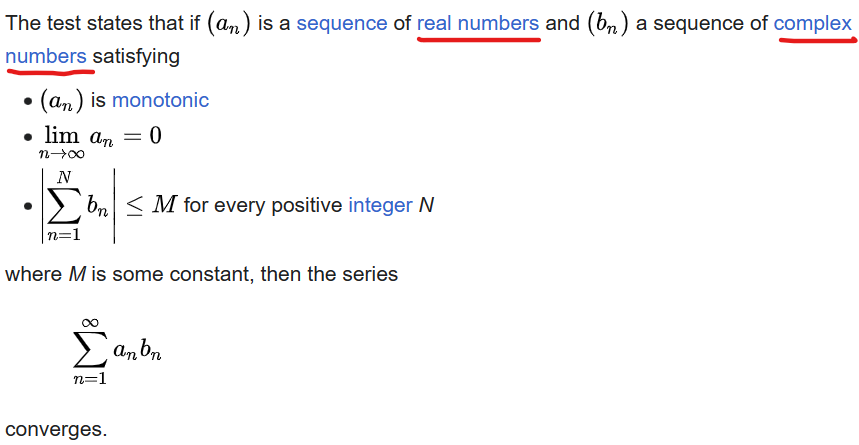
\includegraphics[width=.68\columnwidth]{figure/dirichlet.png}
\end{center}

通过上述证明, 我们可以得到\href{https://en.wikipedia.org/wiki/Abel%27s_test#Abel's_test_in_complex_analysis}{复分析中的 Abel's test}.

\begin{center}
  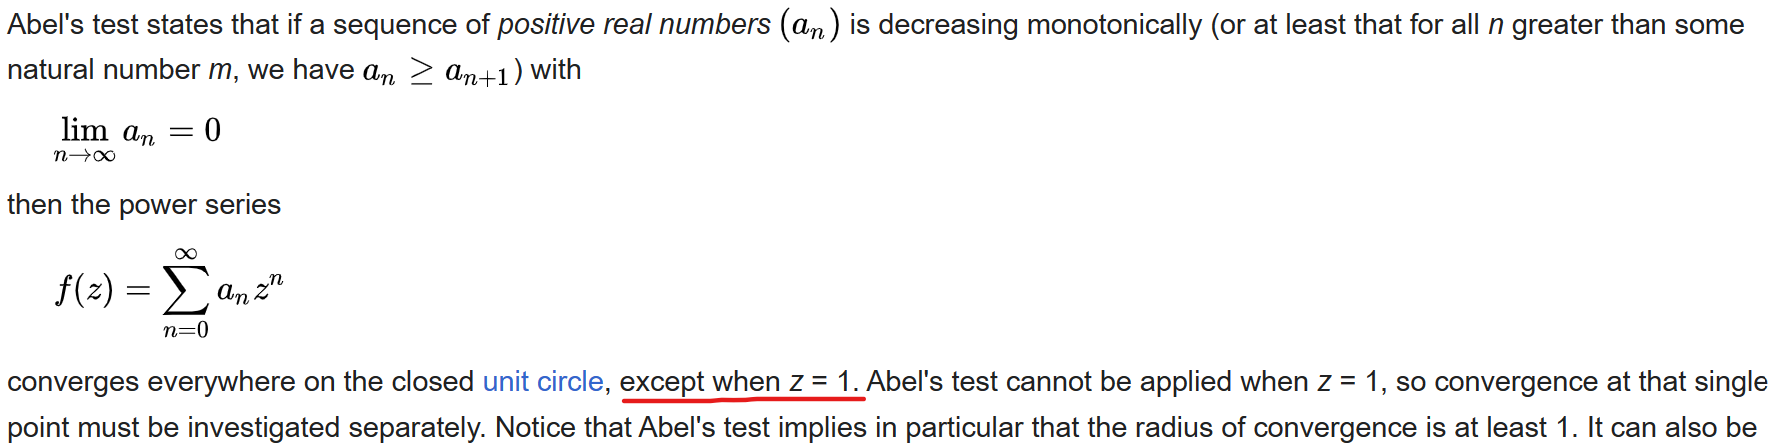
\includegraphics[width=.9\columnwidth]{figure/abel.png}
\end{center}

\question{2}
\subquestion{4}
记收敛半径为 \(R\).
\begin{align*}
  \frac{1}{z^2-3z+2}&=\frac{1}{z-2}-\frac{1}{z-1}\\
  &=-\frac{1}{2}\frac{1}{1-\frac{z}{2}}+\frac{1}{1-z}\\
  &=-\frac{1}{2}\sum_{n=0}^{+\infty}\left(\frac{z}{2}\right)^n+\sum_{n=0}^{+\infty}z^n\\
  &=\sum_{n=0}^{+\infty}\left(1-\frac{1}{2^{n+1}}\right)z^n.
\end{align*}
\(a_n=(1-\frac{1}{2^{n+1}}), r=\lim_{n\to+\infty}|\frac{a_{n+1}}{a_n}|=1, R=\frac{1}{r}=1\).

\subquestion{6}
记收敛半径为 \(R\).
\begin{align*}
  \frac{z}{(1-z)^2}&=z\left(\frac{1}{1-z}\right)'\\
  &=z\left(\sum_{n=0}^{+\infty}z^n\right)'\\
  &=z\sum_{n=0}^{+\infty}nz^{n-1}\\
  &=\sum_{n=0}^{+\infty}nz^n.
\end{align*}
\(a_n=n, r=\lim_{n\to+\infty}|\frac{a_{n+1}}{a_n}|=1, R=\frac{1}{r}=1\).

\subquestion{8}
记收敛半径为 \(R\).
\begin{align*}
  \int_{0}^{z}\frac{\sin z}{z}\,dz&=\int_{0}^{z}\sum_{n=0}^{+\infty}\frac{(-1)^nz^{2n+1}}{(2n+1)!z}\,dz\\
  &=\sum_{n=0}^{+\infty}\frac{(-1)^nz^{2n+1}}{(2n+1)!(2n+1)}.
\end{align*}
\(a_{2n}=0, a_{2n+1}=\frac{(-1)^n}{(2n+1)!(2n+1)}, r=\lim_{n\to+\infty}\sqrt[n]{|a_n|}=0, R=\frac{1}{r}=+\infty\).

\fbox{\parbox{\textwidth}{注释: 上面需要计算 \(\lim_{n\to+\infty}\sqrt[n]{n!}=+\infty\), 除了用 Stirling 公式外, 我们也可以用一些巧法. 注意到 \((n!)^2=(1\cdot n)(2\cdot(n-1))(3\cdot(n-2))\cdots(n\cdot1)\geq n\cdot n\cdot n\cdots n=n^n\), 故 \(\sqrt[n]{n!}\geq\sqrt{n}\).}}

\end{document}